\section{Oxygen-Neon-Magnesium White Dwarf Mergers}
\label{sec:onemg}

Due to their mass, it is likely that the merger of an ONeMg WD with any companion will create a super-Chandrasekhar mass remnant.  The consensus for such mergers is they are more likely to lead to accretion-induced collapse (AIC) than an explosion, though the matter is still not completely resolved \citep{yoonpr07,frye+10,dess+06}.  \cite{taub+11} note an ONeMg triggered to detonate by an ``external event'' may explode instead of collapsing, and mention it as a possible explantion for the very bright ($\sim 10^{43}$ erg s$^{-1}$), slow-decaying SN 2009dc, which apparently ejected over 1.8 {\Msun} of {\Ni} at relatively low kinetic energies.  It is also worthwhile to note that according to Fig. \ref{wdbinarymasses} it is plausible to have an He-ONeMg WD binary whose total mass is below the Chandrasekhar mass, but such a system would interact via stable mass accretion, according to Sec. \ref{ssec:stabilityofmasstransfer}.  From the simulations of \citeauthor{loreig09}, a 0.6 {\Msun} CO - 1.2 {\Msun} ONeMg WD merger will result in carbon nuclear processing, but any runaway nuclear reactions appear to be quenched.  We did not find any simulations of runaway CO burning on an ONeMg WD.

The optical transient of the AIC itself was simulated by \cite{dess+06}.  Their work showed that core collapse results in a shockwave that breaks out along the poles of the (rapidly spinning) WD, followed by a neutrino-driven wind concentrated along the poles that ultimately ejects $3 - 4 \times 10^{-3}$ {\Msun}, depending on the mass of the initial WD, at speeds in the range of 1 - 3 $\times 10^4$ km s$^{-1}$.  About a quarter of the ejected matter is {\Ni}.  The total energy of the explosion is on order $5 \times 10^{49}$ - $10^{50}$ erg.  The time before gamma rays can escape the ejecta is short, and in all this is not a strong optical transient compared to SNe \citep{metz+09}.  Note that earlier work by \cite{frye+99} predicted an order of magnitude higher total mass, energy and $^{56}$Ni.

\cite{metz+09} propose a transient from a different source: following the AIC, the proto-neutron star will be surrounded by a $\sim 0.1$ - $0.5$ {\Msun} Keplerian disk with an outer radius of $\sim30$ - $100$ km and a temperature in the MeV range.  The disk will, due to MHD turbulence, hyper-accrete onto the NS at rates of up to $\sim$ 1 {\Msun} s$^{-1}$; by conservation of momentum, part of the disk will be ejected.  This disk will be proton-rich when it cools to below 1 MeV, and is efficiently synthesized into $^{56}$Ni.  \citeauthor{metz+09} calculate $3 \times 10^{-2}$ {\Msun} of ejecta, about a third of which is $^{56}$Ni, forming by this process from a $\sim 0.1$ {\Msun} accretion disk.  This outflow has similar energies and speeds ($\sim$ 10$^{50}$ erg, $\sim$ 30,000 km s$^{-1}$) to the AIC ejecta \citep{metz+09}.  The light curve from this transient, which they call a ``naked AIC transient'' is shown in Fig. \ref{AICtrans}.

\citeauthor{metz+09} note that for a double-degenerate merger leading to an AIC, significant amounts ($\sim 0.1$ {\Msun}) of WD material will remain in a thick torus at a radius of $10^4$ km.  When the AIC ejecta and accretion disk outflow strike this outer envelope, ejecta speeds will slow from $3 \times 10^4$ km s$^{-1}$ to $3$ - $10 \times 10^3$ km s$^{-1}$ while shock-heating the outer envelope up to $10^9$ K, which synthesizes intermediate mass elements.  The larger total ejecta mass and slower ejecta velocities increase the rise time of the transient from 1 day (the naked case) to $\sim 10$ days, as seen in Fig. \ref{AICtrans} \citep{metz+09}.  In addition to iron-peak elements, the AIC outflow should contain Cr, Kr, Se and Br (not commonly found in SNe), and interactions with the torus should add more intermediate elements which may, in total, constitute a spectrum unique to AICs \citep{metz+09}.  The exact composition of the ejecta will depend on the composition of the WD that merged with the ONeMg WD, and therefore composition could distinguish the difference between an He, CO and ONeMg-ONeMg merger.

\cite{frye+09} simulated an enshrouded AIC at the centre of a merger remnant using a radiation-hydrodynamics code and values similar to \citeauthor{dess+06} ($2 \times 10^{50}$ erg total energy, $0.02$ {\Msun} ejecta, $4 \times 10^{-3}$ {\Msun} {\Ni}), and obtain a similar light curve to \citeauthor{metz+09}'s schematic light curve (Fig. \ref{AICtrans}).  A peak V-band magnitude of -16 was achieved in $\sim$ 10 days.  \cite{frye+09} also simulate an explosion with ten times the energy, mass and {\Ni} in accordance with \cite{frye+99}, and obtain a peak V-band magnitude of -18.5, achieved also in $\sim$ 10 days.  In neither explosion do they recover line features that would be unique to AICs in the resulting spectrum.  They also note that the high energies and low ejecta masses mean most of the ejecta is ionized and line emission is washed out - this occurs early on for their more powerful explosion, and after peak light for their weaker explosion.

\textbf{MARTEN}: It's not clear from literature why the spectral features of Cr, Kr, Se and Br speculated by \citeauthor{metz+09} are not recovered in \cite{frye+09}'s spectra.  It's not really stated by \cite{frye+09}, though they most certainly know \citeauthor{metz+09}'s work.  You might also want to use \citeauthor{frye+09}'s spectrum instead of the schematic from \citeauthor{metz+09}.

\begin{figure}
\centerline{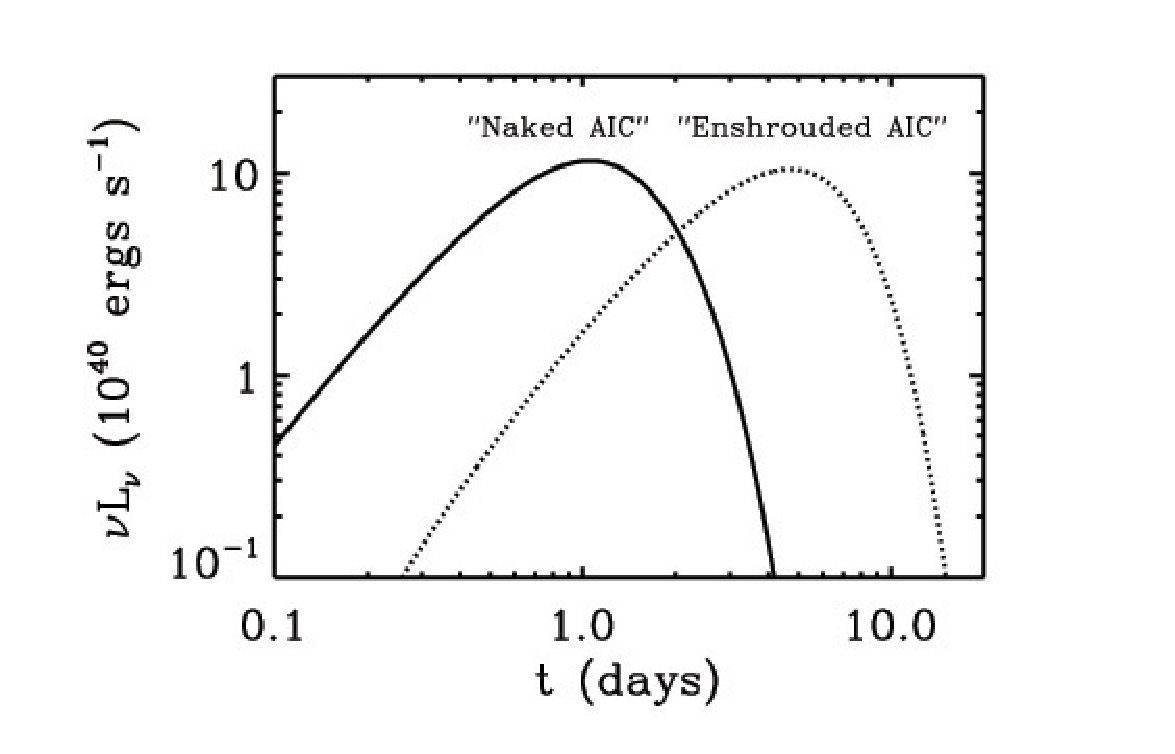
\includegraphics[width=0.8\hsize]{AICtrans.pdf}}
\caption{Model V-band light curve of two AIC transients.  The naked transient (total mass $2 \times 10^{-2}$ {\Msun}, $10^{-2}$ {\Msun} $^{56}$Ni, $v = 3 \times 10^4 km s^{-1}$), resulting from a stable mass transfer AIC, does not have an envelope left over from a WD merger, and rises and falls within a day's time.  The enshrouded AIC transient (total mass $2 \times 10^{-1}$ {\Msun}, $10^{-2}$ {\Msun} $^{56}$Ni, $v = 10^4 km s^{-1}$) results from a WD merger, and therefore as an envelope that stretches out the light curve over a week while keeping peak luminosity constant.  These curves are consistent with \cite{frye+09}'s Fig. 7.  From \cite{metz+09}, their Fig. 2.}
\label{AICtrans}
\end{figure}

Such an ``enshrouded AIC'' transient could be responsible for SN 2008ha, whose rise time, peak luminosity, ejecta velocity, ejected mass and ejected {\Ni} are all within range of the corresponding values stated above.  With 0.16 {\Msun} ejected at speeds of $\sim 10^4$ km s$^{-1}$ and $\sim 0.02$ {\Msun} {\Ni} produced, and possible detection of Al II lines in its spectrum, SN 2010X is also an enshrouded AIC candidate \citep{kasl+10}.  It is not likely for this merger channel to explain all possible sub-luminous SNe Ia, as most others eject much more $^{56}$Ni than can be formed from an AIC-related transient \citep{fole+09}.

If the WD merger remnant rotates differentially, then any initial poloidal magnetic field will be greatly amplified through the magnetorotational instability.  \cite{dess+07} show that the entire star consequently spins down by as much as 30\%, and the rotational energy lost is fed into a magnetically driven wind substantially more powerful than the neutrino wind described above.  Explosion energies then reach up to $\sim 10^{51}$ erg and $\sim$ 0.1 {\Msun} is ejected, though negligble amounts of {\Ni} are created.  The transient, therefore, is still fairly weak optically, and could instead be detected via neutrino and gravitational wave emission \citep{dess+07}.

\citeauthor{metz+09} also speculate as to whether an AIC could emit a collimated relativistic outflow, thereby creating a short gamma-ray burst.  One advantage to AIC-GRBs is that the late-time (around 10 - 100 s) x-ray tail seen in some short GRBs could plausibly be explained by late-time accretion of merger remnant material not carried away by the initial AIC outflow, or by magnetar outflows (assuming one is created by an AIC).  See \cite{dess+07}, however, for discussion as to why AICs likely will not create short GRBs unless the collapsing WD eventually forms a black hole.  This 10 - 100 s x-ray emission might be seen regardless, and could be a target for x-ray survey missions \citep{metz+09}.

%WHY IS TOTAL ENERGY GREATER IN ENSHROUDED CASE?

%-Nucleosythetically speaking, could an ONeMg WD create an SN Ia?  I.e. the ejecta composition should be different, but in what way?  Fairly sure the answer's no - see Taubenberger on ONeMg explosion speculation.